% SPDX-License-Identifier: AGPL-3.0-or-later
% Copyright (C) 2019 Andrew Rechnitzer
% Copyright (C) 2023 Colin B. Macdonald

\documentclass[12pt]{article}

\usepackage{tikz}
\usetikzlibrary{backgrounds}

\begin{document}
\thispagestyle{empty}
\begin{center}
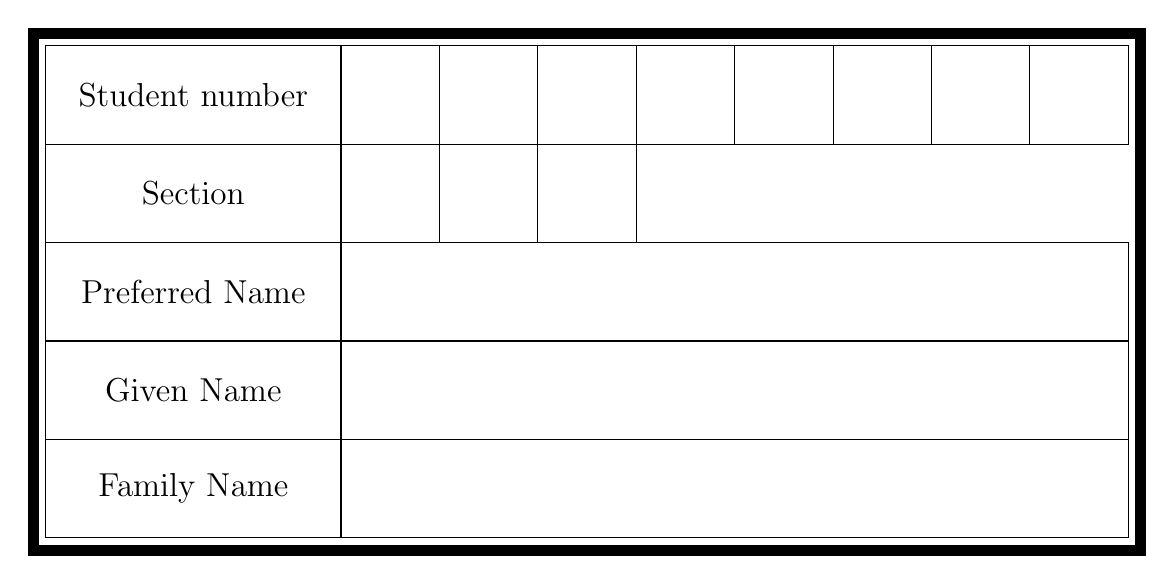
\begin{tikzpicture}[scale=1.25, background rectangle/.style={line width=4pt, draw=black}, show background rectangle]
  \draw (0,1) rectangle (3,2) node[pos=0.5] {\large Family Name}; \draw (3,1) rectangle (11,2);
  \draw (0,2) rectangle (3,3) node[pos=0.5] {\large Given Name}; \draw (3,2) rectangle (11,3);
  \draw (0,3) rectangle (3,4) node[pos=0.5] {\large Preferred Name}; \draw (3,3) rectangle (11,4);

  \draw (0,4) rectangle (3,5) node[pos=0.5] {\large Section};
  \foreach \x in {0,...,2} {
    \draw (\x+3,4) rectangle (\x+4,5);
  }

  \draw (0,5) rectangle (3,6) node[pos=0.5] {\large Student number};
  \foreach \x in {0,...,7} {
    \draw (\x+3,5) rectangle (\x+4,6);
  }
\end{tikzpicture}
\end{center}

\end{document}
